\documentclass[a0]{sciposter}
\usepackage[spanish]{babel}
\usepackage{multicol}
\usepackage{amsmath, amssymb, fontspec, lipsum,caption}
\usepackage{graphicx,float,hyperref}  
\usepackage{dcolumn}   
\usepackage{bm}        
\usepackage{graphicx}
\usepackage{tabularx}
\usepackage{multirow}
\usepackage{booktabs}
\usepackage{textcomp} 
\usepackage[linesnumbered,algoruled,longend]{algorithm2e}
\setromanfont[
BoldFont=QuattrocentoSans-Bold.ttf,
ItalicFont=QuattrocentoSans-BoldItalic.ttf,
BoldItalicFont=QuattrocentoSans-Italic.ttf
]{QuattrocentoSans-Regular.ttf}
\setsansfont[
BoldFont=QuattrocentoSans-Bold.ttf,
ItalicFont=QuattrocentoSans-BoldItalic.ttf,
BoldItalicFont=QuattrocentoSans-Italic.ttf
]{QuattrocentoSans-Regular.ttf}
\newcommand{\midsepremove}{\aboverulesep = 0mm \belowrulesep = 0mm}
\midsepremove
\newcommand{\midsepdefault}{\aboverulesep = 0.605mm \belowrulesep = 0.984mm}
\midsepdefault
\title{Simulación de Propiedades Mecánicas de Carbono Amorfo}
\author{\underline{Daniel Castillo}$^1$ and Rafael I. Gonz\'alez$^{2,3}$}
\institute 
{$^1$Centro de \'Optica e Informaci\'on Cu\'antica, Universidad Mayor, Santiago, Chile.\\$^2$Centro de Nanotecnolog\'ia Aplicada, Universidad Mayor, Santiago, Chile.\\$^2$Centro para el Desarrollo de la Nanociencia y la Nanotecnolog\'ia, CEDENNA, Santiago, Chile.}
\email{{daniel.castilloca, rafael.gonzalezvaldes}{(@mayor.cl})}
\leftlogo[0.7]{chimex.png}
\rightlogo[0.7]{uma.png}
\begin{document}
\maketitle
\newcommand{\mycaption}{%
\ifx \@captype \@undefined \@latex@error {\noexpand \caption outside float}\@ehd \expandafter \@gobble \else \refstepcounter \@captype \expandafter \@firstofone \fi {\@dblarg {\@caption \@captype }}
}
\begin{multicols}{2}
\section{Introducción}
\begin{itemize}
\item La realización de centros de color en carbono amorfo, material que tiene una estructura química entre grafito y diamante, ha generado un gran interés de investigación reciente.\\ \item Se ha demostrado una relación directa entre procesos de Información Cuántica y de Termodinámica Cuántica. En principio porque ambas teorías comparten el concepto de entropía.
\end{itemize}
\section{Método}
\begin{itemize}
\item Se hicieron simulaciones de dinámica molecular clásica usando el programa LAMMPS con diferentes potenciales de interacci\'on. \cite{Lammps}.\\
\item de Tom\'as {\it et al.}\cite{ACPot1} propusieron un método para obtener muestras de carbono amorfo a partir de un arreglo cúbico de átomos de carbono que son calentados y enfriados en un proceso extremadamente r\'apido.\\
\item Se obtuvieron muestras de carbono amorfo, las que fueron caracterizadas tanto por su densidad como la relaci\'on sp$^2$/sp$^3$. Se estudi\'o la evoluci\'on de las muestras con la temperatura y se calcul\'o el módulo de bulto.
\end{itemize}
\begin{figure}
        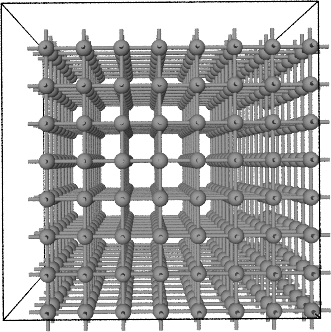
\includegraphics[width=0.4\textwidth]{carbon1.png}
        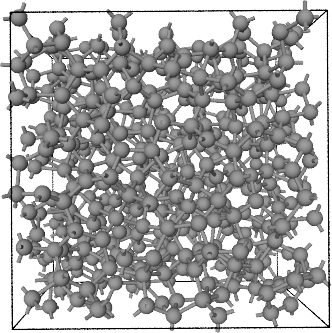
\includegraphics[width=0.4\textwidth]{carbon2.png}
    \label{fig:carbon}
\end{figure}
\section{Resultados y Análisis}
\begin{itemize}
\item  Se observa un cambio de fase estructural a grafito estructural, que está de acuerdo con la derivación sobre las fases del carbono hecha en \cite{Zazula}. \\
\end{itemize}
  \begin{figure}
        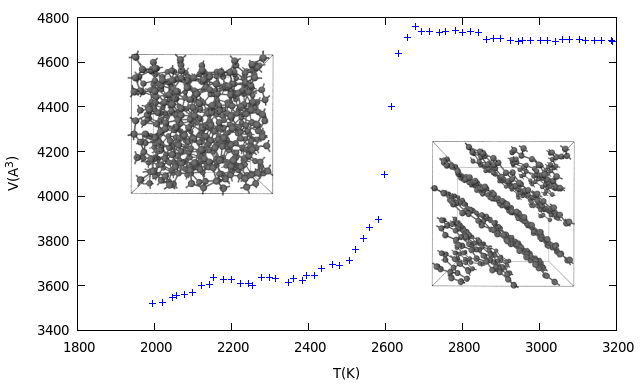
\includegraphics[width=0.95\textwidth]{melting.png}
        \label{fig:meltproc}
\end{figure}
\begin{itemize}
\item Se trabajó con potenciales mencionados por de Tom\'as {\it et al.} \cite{ACPot1}, tales como REBOII, AIREBO, BOP, EDIP y ReaxFF.\\
\item La medición de los puntos de cambio de fase para todas las muestras se obtuvo observando la dinámica dentro de la muestra usando el programa de visualizaci\'on y An\'alisis OVITO \cite{Ovito}. \\
\item Se observa que la temperatura en que comienza el cambio de fase se reduce con el aumento de \'atomos con enlaces tipo sp$^3$, es decir, muestras m\'as cercanas a diamante.\\ 
\end{itemize}
\begin{figure}
        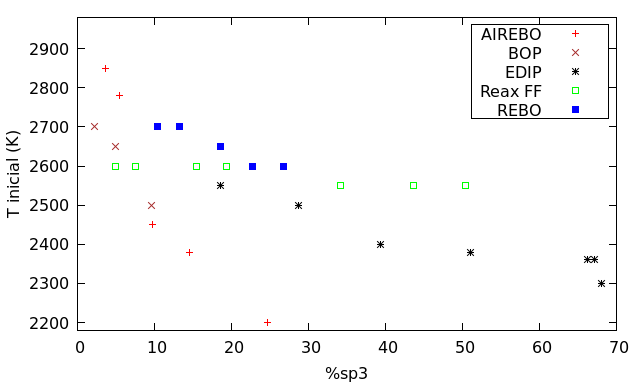
\includegraphics[width=0.95\textwidth]{datamelting.png}
        \label{fig:meltdata}
\end{figure}

\begin{itemize}
    \item El m\'odulo de bulto de diferentes muestras se obtienen en simulaciones computancionales donde se calcu\'o la presi\'on del sistema como funci\'on del volumen de la muestra. La muestra se comprime y luego se expande de manera lenta.\\
\item El módulo de bulto se obtiene relacionando la presión y el volumen medidos en cada muestra, tal como se ve en el gr\'afico siguiente. \\
\end{itemize}
\begin{figure}
        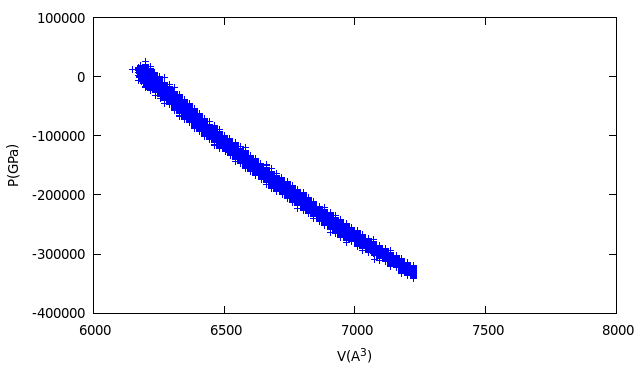
\includegraphics[width=0.95\textwidth]{bulk.png}
        \label{fig:bulkproc}
\end{figure}
\begin{itemize}
    \item Abajo se resume el m\'odulo de bulto obtenido como funci\'on del \% de sp$^3$ de  las muestras para diferentes potenciales. A grandes razgos, se puede indicar que se obtuvieron valores entre 100 y 300 GPa  lo que concuerda con el trabajo de \cite{RefBulk} que sugiere valores entre los 200 y 350 GPa. \\
    \end{itemize}

\begin{figure}
        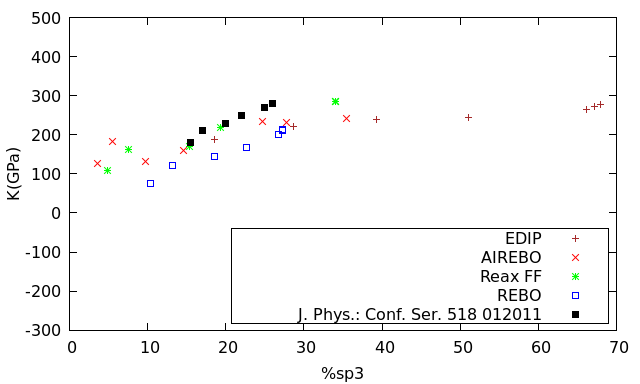
\includegraphics[width=0.95\textwidth]{databulk.png}
        \label{fig:bulkdata}
\end{figure}

\section{Conclusiones}
\begin{itemize}
    \item  Se generaron muestras de carbono amorfo de diferentes densidades con potenciales de interacci\'on que son ampliamente utilizados en simulaciones de materiales en base a carbono. \\
    \item  Para la mayor\'ia de potenciales de interacci\'on se encontraron rangos de densidades  (\% de sp$^3$) en que el m\'odulo de bulto es cercano al reportado en la literatura.\\
 
 
    \item Proyecciones: insertar defectos propios de centros de color en carbono amorfo con alto \% de sp$^3$, evaluar más propiedades termodinámicas y vibracionales. Evaluar dichos sistemas usando formalismos más sofisticados como DFT.\\ 
\end{itemize}

%%% References
\begin{thebibliography}{99}
\bibitem{Lammps} S. Plimpton, J Comp Phys 117, 1-19 (1995).
\bibitem{ACPot1} C. De Tomás, I. Suarez-Martínez ,N. Marks, Carbon 109,681-693 (2016).
\bibitem{Zazula} J. M. Zazula, LHC Project Note 87 (1997).
\bibitem{Ovito} A. Stukowski, Matter. Sci. Eng. 18, 015012 (2010).
\bibitem{RefBulk} A. M. Ito, A. Takayama, Y. Oda, H. Nakamura, J. Phys.: Conf. Ser. 518, 012011 (2014).
\end{thebibliography}

\section{Agradecimientos}
D.C. agradece la beca doctoral de la Universidad Mayor. R.I.G. agradece el apoyo de FONDECYT con el proyecto \# 11180557 y a CEDENNA.

\end{multicols}
\end{document}
